\section{Αρχιτεκτονική σχεδίαση} \label{section:3-7-architecture-design}

Στο κεφάλαιο αυτό περιγράφεται η αρχιτεκτονική του συστήματος, όπως προέκυψε από την επιλεγμένη τεχνολογική στοίβα και τις προαναφερθείσες απαιτήσεις του. Θα πρέπει να σημειωθεί ότι η αρχιτεκτονική αυτή είναι πρώιμη και δεν αποτελεί την τελική υλοποίηση της πλατφόρμας, η οποία περιγράφεται στο κεφάλαιο \ref{chapter:4-application-implementation}. 

Συνοπτικά, η αρχιτεκτονική του συστήματος αποτυπώνεται στο παρακάτω διάγραμμα:

% TODO: Add proper figure
\begin{figure}[H]
    \centering
    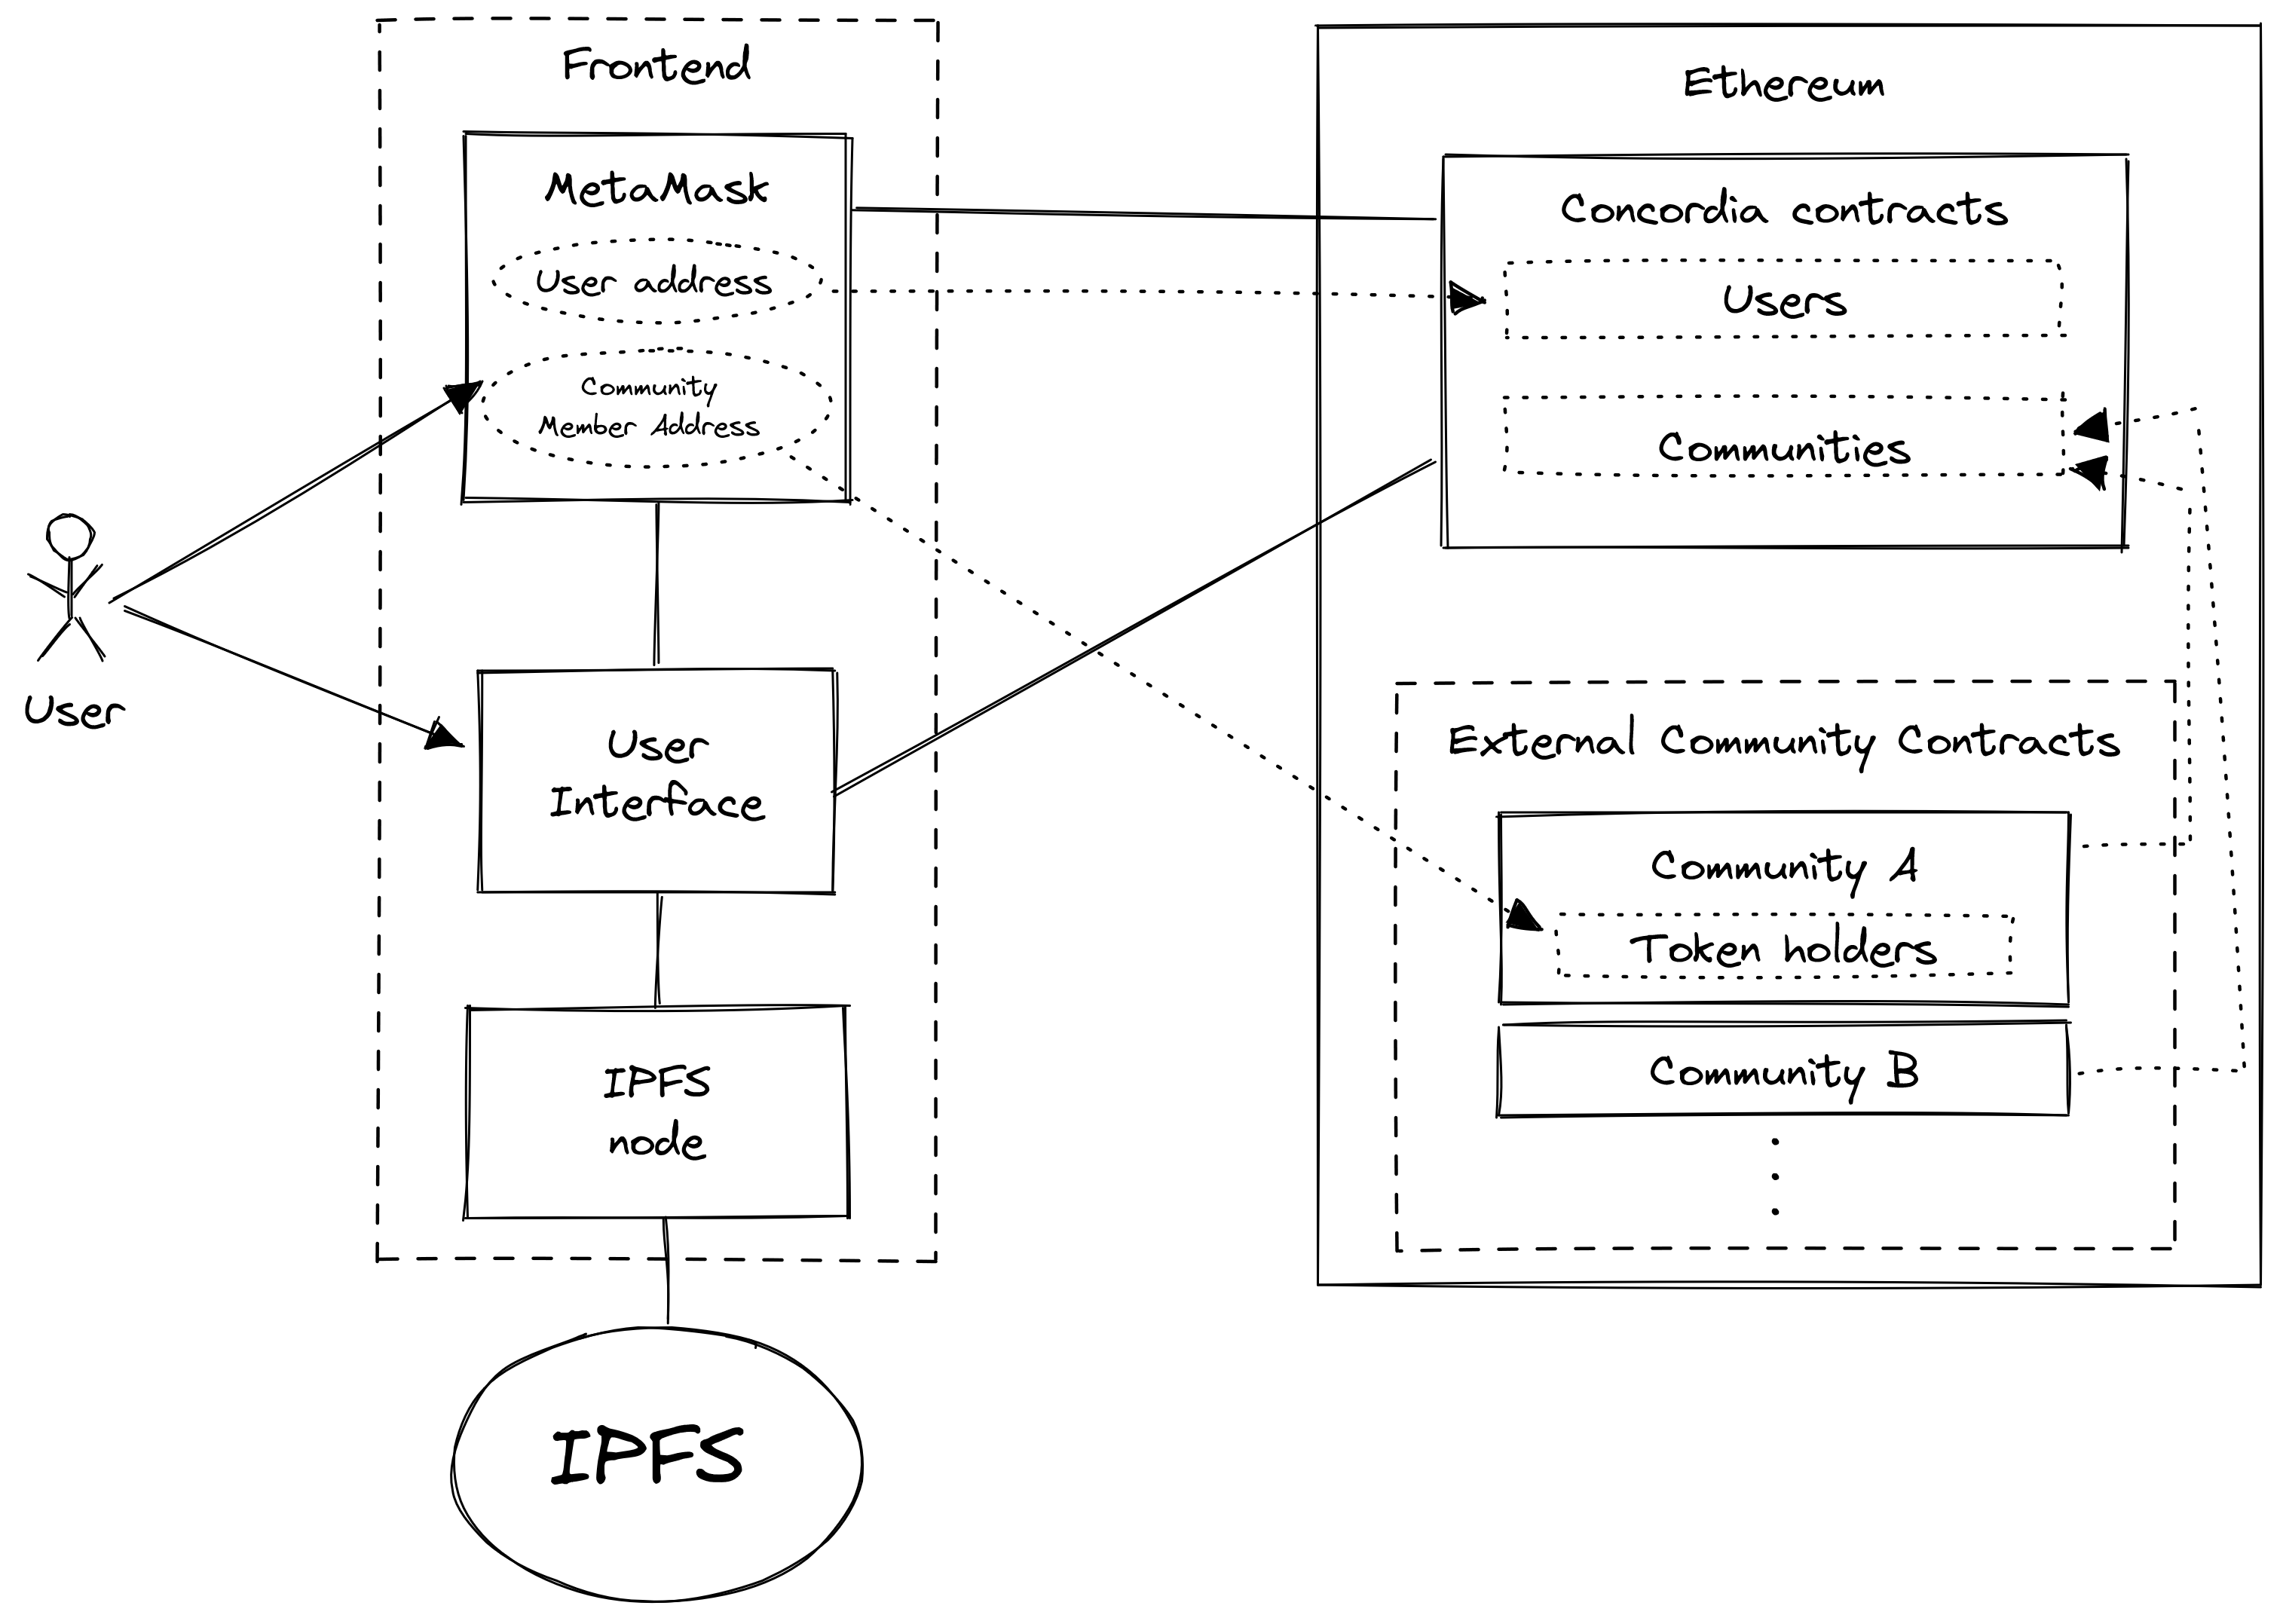
\includegraphics[width=.75\textwidth]{assets/figures/chapter-3/3.7.architecture-design}
    \caption{Αρχιτεκτονική του συστήματος (στάδιο σχεδίασης)}
\end{figure}

% TODO: Explain diagram
